% This file is a template using the "beamer" package to create slides for a talk or presentation
% - Talk at a conference/colloquium.
% - Talk length is about 20min.
% - Style is ornate.


% draft包的作用是在编译时不生成目录,这样可以在编辑文档查看效果时加快编译速度,但是在确定文档内容后,需要删除draft包(使用下一行documentclass),否则目录不会生成。
% \documentclass[aspectratio=169, UTF8, draft]{beamer}
\documentclass[aspectratio=169, UTF8]{beamer}

\usepackage{ctex}

\mode<presentation>
{
  \usetheme{Kokura}
}


\usepackage[english]{babel}
% or whatever


% 在封面页需要展示的信息
\title{\textbf{基于Cesium的实景三维专题表达方法研究}}
\subtitle{一份毕业答辩Beamer演示文稿} % 可选
\author{Falldio}
\institute{武汉大学资源与环境科学学院}
\date{1999年5月23日}

% Delete this, if you do not want the table of contents to pop up at
% the beginning of each subsection:
% \AtBeginSubsection[]
% {
  % \begin{frame}<beamer>{Outline}
    % \tableofcontents[currentsection,currentsubsection]
  % \end{frame}
% }

\begin{document}
% 默认在title page中加入图片background.png
{
  \usebackgroundtemplate{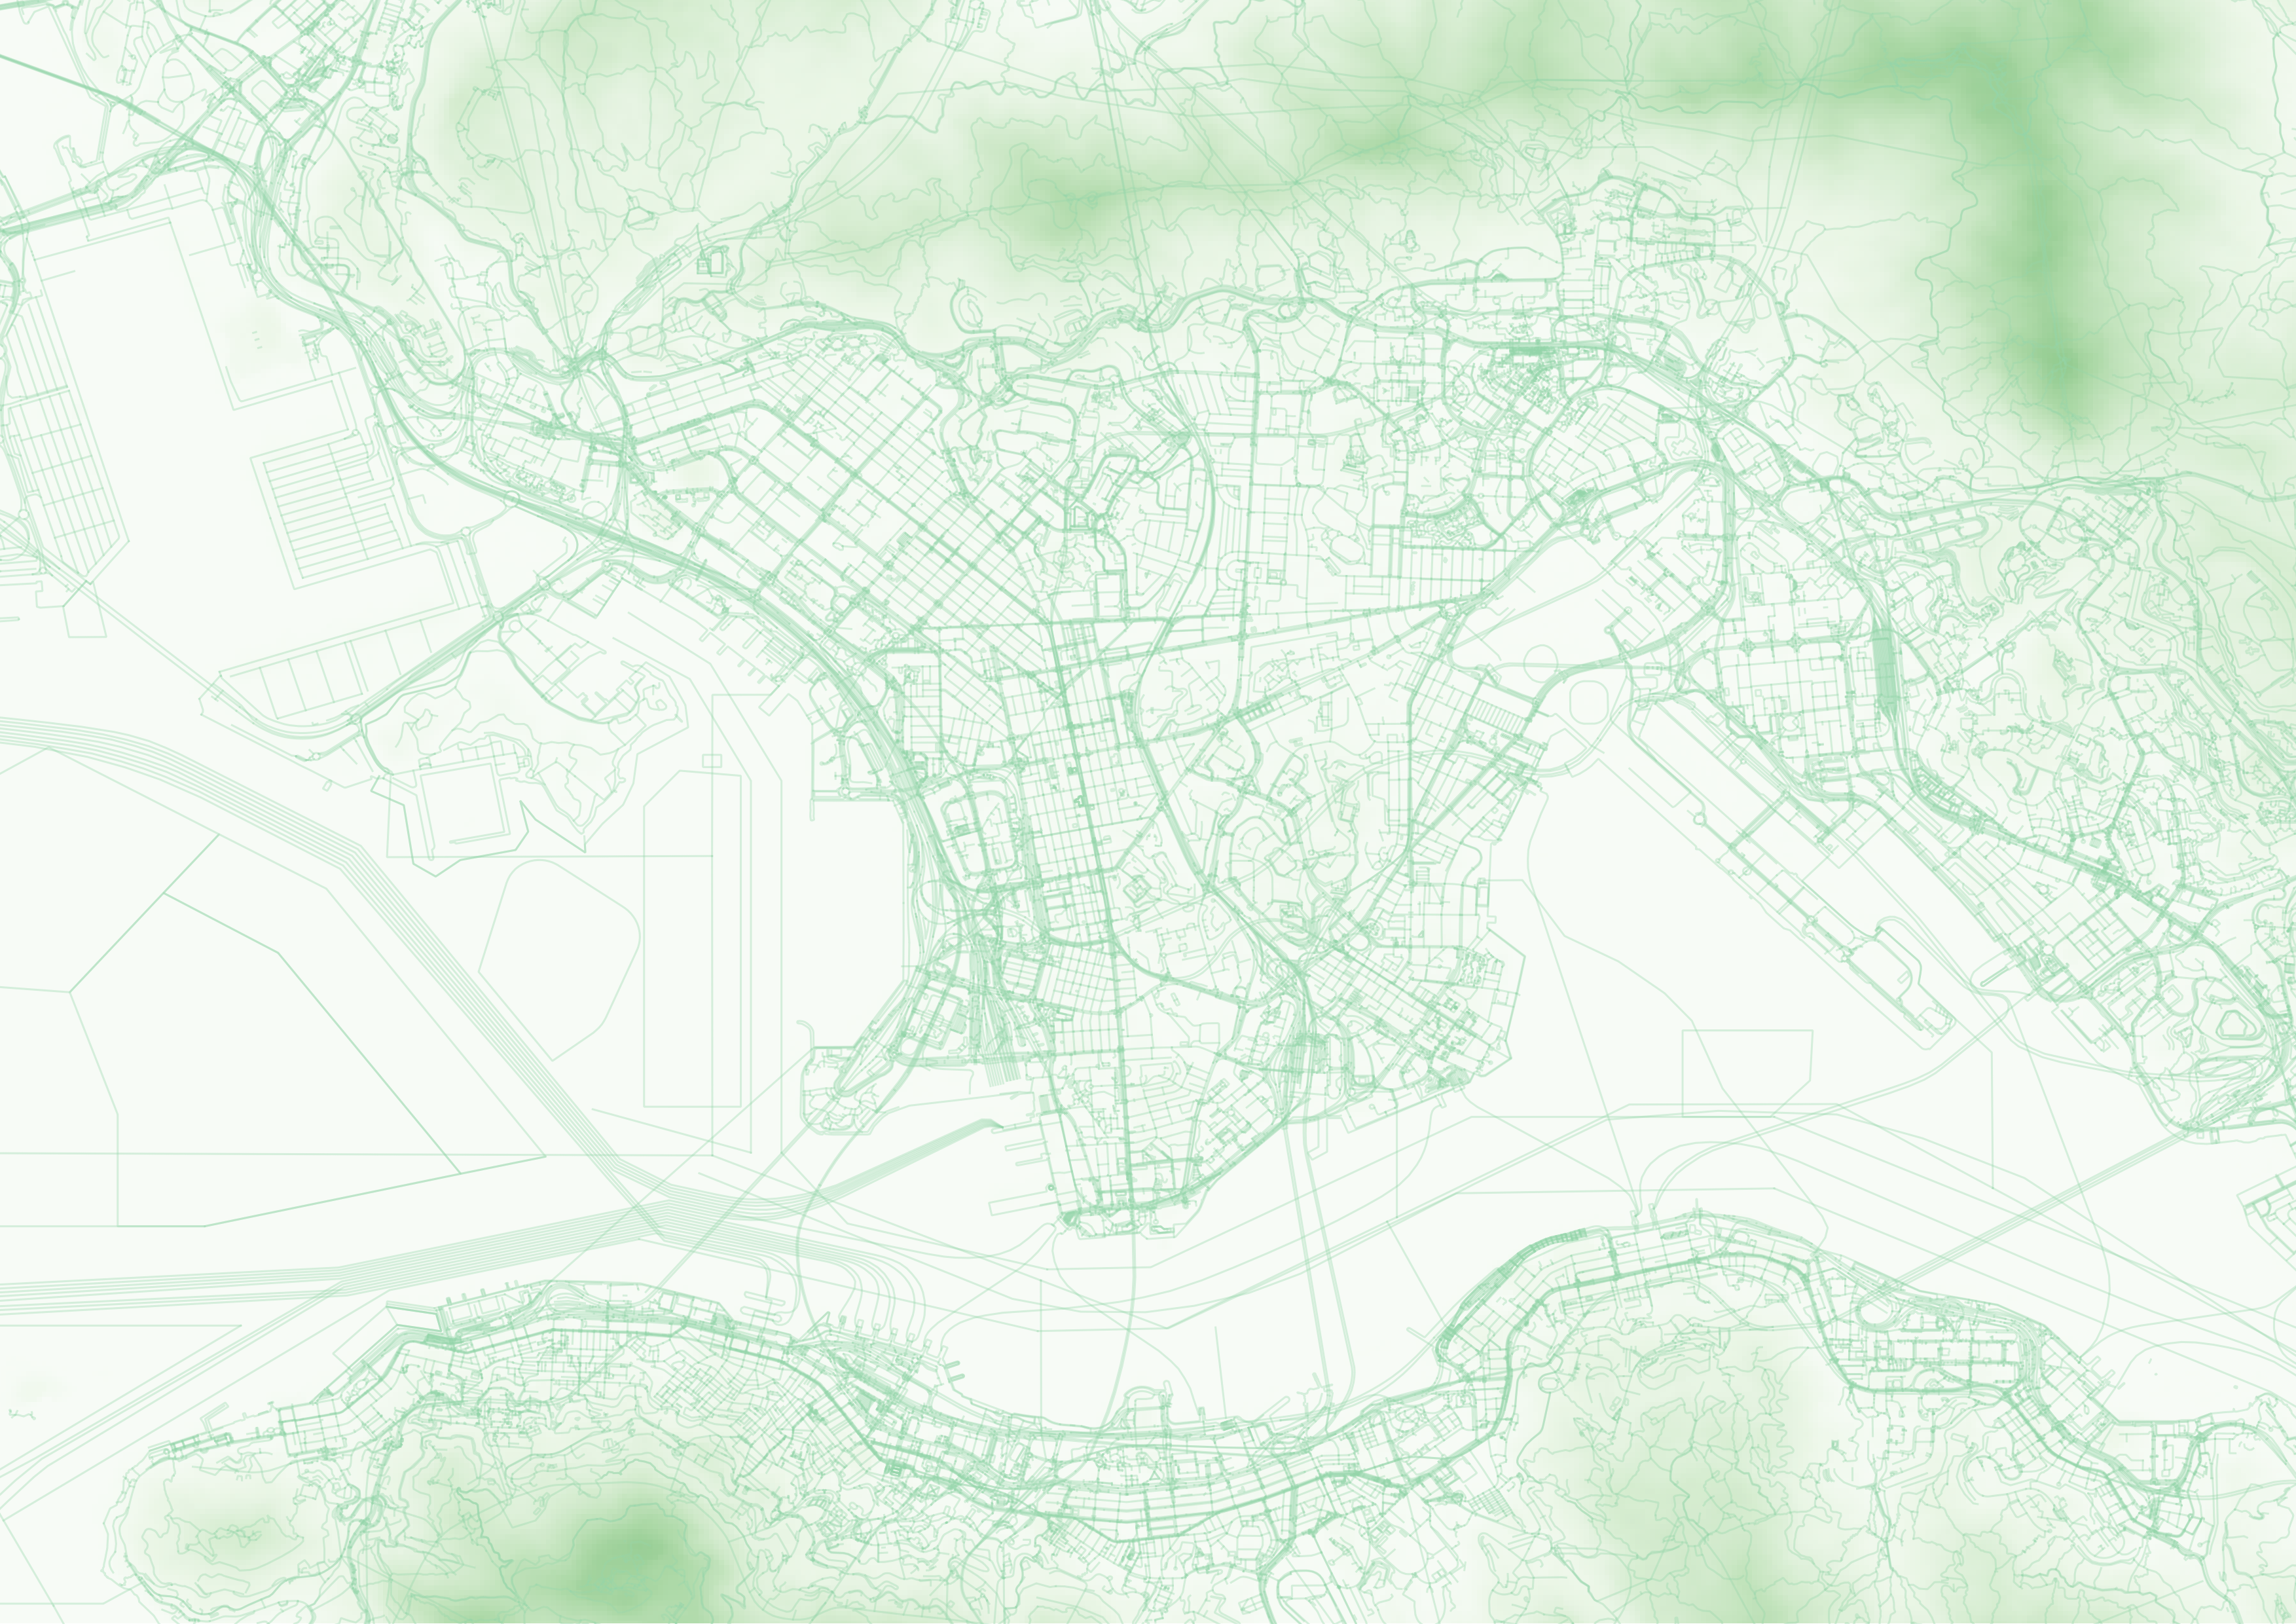
\includegraphics[width=\paperwidth]{background.png}} % 背景图片
  \begin{frame}[plain, noframenumbering]
    \titlepage
  \end{frame}
}

% 如果不需要背景图片,可以使用下面的命令
% \begin{frame}[plain, noframenumbering]
  % \titlepage
% \end{frame}

\begin{frame}{Outline}
  \tableofcontents
  % You might wish to add the option [pausesections]
\end{frame}

\section{Motivation}

\subsection{The Basic Problem That We Studied}

\begin{frame}{Make Titles Informative. Use Uppercase Letters.}{Subtitles are optional.}
  % - A title should summarize the slide in an understandable fashion
  %   for anyone how does not follow everything on the slide itself.

  \begin{itemize}
  \item
    Use \texttt{itemize} a lot.
  \item
    Use very short sentences or short phrases.
  \end{itemize}
\end{frame}

\begin{frame}{Make Titles Informative.}

  You can create overlays\dots
  \begin{itemize}
  \item using the \texttt{pause} command:
    \begin{itemize}
    \item
      First item.
      \pause
    \item    
      Second item.
    \end{itemize}
  \item
    using overlay specifications:
    \begin{itemize}
    \item<3->
      First item.
    \item<4->
      Second item.
    \end{itemize}
  \item
    using the general \texttt{uncover} command:
    \begin{itemize}
      \uncover<5->{\item
        First item.}
      \uncover<6->{\item
        Second item.}
    \end{itemize}
  \end{itemize}
\end{frame}


\subsection{Previous Work}

\begin{frame}{Make Titles Informative.}
\end{frame}

\begin{frame}{Make Titles Informative.}
\end{frame}



\section{Our Results/Contribution}

\subsection{Main Results}

\begin{frame}{Make Titles Informative.}
\end{frame}

\begin{frame}{Make Titles Informative.}
\end{frame}

\begin{frame}{Make Titles Informative.}
\end{frame}


\subsection{Basic Ideas for Proofs/Implementation}

\begin{frame}{Make Titles Informative.}
\end{frame}

\begin{frame}{Make Titles Informative.}
\end{frame}




\section*{Summary}

\begin{frame}{Summary}

  % Keep the summary *very short*.
  \begin{itemize}
  \item
    The \alert{first main message} of your talk in one or two lines.
  \item
    The \alert{second main message} of your talk in one or two lines.
  \item
    Perhaps a \alert{third message}, but not more than that.
  \end{itemize}
  
  % The following outlook is optional.
  \vskip0pt plus.5fill
  \begin{itemize}
  \item
    Outlook
    \begin{itemize}
    \item
      Something you haven't solved.
    \item
      Something else you haven't solved.
    \end{itemize}
  \end{itemize}
\end{frame}



% All of the following is optional and typically not needed. 
\appendix
\section<presentation>*{\appendixname}
\subsection<presentation>*{For Further Reading}

\begin{frame}[allowframebreaks]
  \frametitle<presentation>{For Further Reading}
    
  \begin{thebibliography}{10}
    
  \beamertemplatebookbibitems
  % Start with overview books.

  \bibitem{Author1990}
    A.~Author.
    \newblock {\em Handbook of Everything}.
    \newblock Some Press, 1990.
 
    
  \beamertemplatearticlebibitems
  % Followed by interesting articles. Keep the list short. 

  \bibitem{Someone2000}
    S.~Someone.
    \newblock On this and that.
    \newblock {\em Journal of This and That}, 2(1):50--100,
    2000.
  \end{thebibliography}
\end{frame}

\end{document}


